\documentclass{beamer}\usepackage{graphicx, color}
%% maxwidth is the original width if it is less than linewidth
%% otherwise use linewidth (to make sure the graphics do not exceed the margin)
\makeatletter
\def\maxwidth{ %
  \ifdim\Gin@nat@width>\linewidth
    \linewidth
  \else
    \Gin@nat@width
  \fi
}
\makeatother

\IfFileExists{upquote.sty}{\usepackage{upquote}}{}
\definecolor{fgcolor}{rgb}{0.2, 0.2, 0.2}
\newcommand{\hlnumber}[1]{\textcolor[rgb]{0,0,0}{#1}}%
\newcommand{\hlfunctioncall}[1]{\textcolor[rgb]{0.501960784313725,0,0.329411764705882}{\textbf{#1}}}%
\newcommand{\hlstring}[1]{\textcolor[rgb]{0.6,0.6,1}{#1}}%
\newcommand{\hlkeyword}[1]{\textcolor[rgb]{0,0,0}{\textbf{#1}}}%
\newcommand{\hlargument}[1]{\textcolor[rgb]{0.690196078431373,0.250980392156863,0.0196078431372549}{#1}}%
\newcommand{\hlcomment}[1]{\textcolor[rgb]{0.180392156862745,0.6,0.341176470588235}{#1}}%
\newcommand{\hlroxygencomment}[1]{\textcolor[rgb]{0.43921568627451,0.47843137254902,0.701960784313725}{#1}}%
\newcommand{\hlformalargs}[1]{\textcolor[rgb]{0.690196078431373,0.250980392156863,0.0196078431372549}{#1}}%
\newcommand{\hleqformalargs}[1]{\textcolor[rgb]{0.690196078431373,0.250980392156863,0.0196078431372549}{#1}}%
\newcommand{\hlassignement}[1]{\textcolor[rgb]{0,0,0}{\textbf{#1}}}%
\newcommand{\hlpackage}[1]{\textcolor[rgb]{0.588235294117647,0.709803921568627,0.145098039215686}{#1}}%
\newcommand{\hlslot}[1]{\textit{#1}}%
\newcommand{\hlsymbol}[1]{\textcolor[rgb]{0,0,0}{#1}}%
\newcommand{\hlprompt}[1]{\textcolor[rgb]{0.2,0.2,0.2}{#1}}%

\usepackage{framed}
\makeatletter
\newenvironment{kframe}{%
 \def\at@end@of@kframe{}%
 \ifinner\ifhmode%
  \def\at@end@of@kframe{\end{minipage}}%
  \begin{minipage}{\columnwidth}%
 \fi\fi%
 \def\FrameCommand##1{\hskip\@totalleftmargin \hskip-\fboxsep
 \colorbox{shadecolor}{##1}\hskip-\fboxsep
     % There is no \\@totalrightmargin, so:
     \hskip-\linewidth \hskip-\@totalleftmargin \hskip\columnwidth}%
 \MakeFramed {\advance\hsize-\width
   \@totalleftmargin\z@ \linewidth\hsize
   \@setminipage}}%
 {\par\unskip\endMakeFramed%
 \at@end@of@kframe}
\makeatother

\definecolor{shadecolor}{rgb}{.97, .97, .97}
\definecolor{messagecolor}{rgb}{0, 0, 0}
\definecolor{warningcolor}{rgb}{1, 0, 1}
\definecolor{errorcolor}{rgb}{1, 0, 0}
\newenvironment{knitrout}{}{} % an empty environment to be redefined in TeX

\usepackage{alltt}
\usetheme{Stats}
\setbeamercovered{transparent}
\usepackage{color}
\usepackage{hyperref}
  \hypersetup{
  	colorlinks=true
		linkcolor=black
		}
\usepackage{url}
\usepackage{graphics}
\usepackage{tikz}
\usepackage{booktabs}





%%%%%%%%%%%%%%%%%%%%%%%%%%%%%%%% Title Slide %%%%%%%%%%%%%%%%%%%%%%%%%%
\title[]{Intro to Social Science Data Analysis \\[1cm] Lecture 6: Data Visualisation in R}
\author[]{
    \href{mailto:gandrud@yonsei.ac.kr}{Christopher Gandrud}
}
\date{\today}


\begin{document}

\frame{\titlepage}

\section[Outline]{}
\frame{\tableofcontents}

\section{Assignment 2}
\frame{
  \frametitle{Assignment 2}
  \textbf{Due:} Friday 19 October \\[0.25cm]
  
  \textbf{Describe} at least \textbf{3} variables in a data set.\\[0.25cm]
  {\small{
    You need to select a \textbf{range of descriptive statistical tools}. The tools should include both \textbf{numerical descriptive statistics} and \textbf{graphics}.\\[0.25cm]

    These tools should describe the variables':
    \begin{itemize}
      \item<1-> central tendency,
      \item<1-> variation,
      \item<1-> their relationships with the other variables.
    \end{itemize}

    The descriptions need to be discussed \textbf{in paragraph form}. \\[0.25cm]

    The description must be \textbf{reproducible}. So you should email me the link to a Dropbox folder with:
    \begin{itemize}
      \item<1-> the \texttt{.csv} data set,
      \item<1-> the \texttt{.Rmd} R markdown file,
      \item<1-> the final \texttt{.html} file.
    \end{itemize}
  }}
}

\section{Recap}
\frame{
	\frametitle{Quick Quiz (1)}
  {\Large{When you describe data, what {\bf{two}} things do you always need to discuss? \\[0.5cm]
  
  Why do you need to describe both things? \\[0.5cm]
  
  Give examples for data at different measurement levels.
  }}
}

\frame{
  \frametitle{Quick Quiz (2)}
  {\Large{What is the difference between the {\bf{population}} mean and the {\bf{sampling}} mean? \\[1cm]
  Why would you log transform a variable?
  }}
}

\frame{
  \frametitle{Today}
  {\Large{Last week: we largely learned how to describe our data {\emph{numerically}}. \\[0.5cm]
  {\bf{Today}}: we will learn how to present our data with {\emph{graphics}}. \\[0.25cm]
  We will learn both how to create graphics in R, but also the principles of effective statistical graphics.
  }}
}

\frame{
  \frametitle{Inferential Statistics}
  {\Large{Many of the things we learn today will also apply to inferential statistics.}}
}

\frame{
  \frametitle{}
  {\Large{The first part of this lecture is based on Tufte (2001) \\[0.5cm]
  Many of the examples are from the Junk Charts Blog (\url{http://junkcharts.typepad.com/}). \\[0.5cm]
  We will also use the World Bank data we downloaded last class. \\
  R Source Code at: \url{http://bit.ly/OTWEGS}
  }}


}

%%%%%%%%%%%%%%%%% Principles of Graphical Excellence %%%%%%%%%%%%%
\section{Principles of Graphics Excelence}
\frame{
  \frametitle{Why Graphics?}
  \begin{center}
  {\Large{Why use graphics? Why not just describe all of our data in tables?}}
  \end{center}
}

\begin{frame}[fragile,plain]
\begin{knitrout}
\definecolor{shadecolor}{rgb}{0.969, 0.969, 0.969}\color{fgcolor}\begin{kframe}
\begin{alltt}
\hlcomment{# Create data frame with GDP/Capita & Infant Mort.}
DataDump <- InfantNoMiss[, 
              \hlfunctioncall{c}(\hlstring{"GDPperCapita"}, \hlstring{"InfantMortality"})]

\hlcomment{# Show data}
DataDump
\end{alltt}
\begin{verbatim}
##     GDPperCapita InfantMortality
## 7        38959.8             6.3
## 8          425.1            76.2
## 9        13829.8             7.2
## 10        3795.7            14.1
## 11        2803.3            17.2
## 12        4068.5           100.1
## 13        7665.1            13.4
## 15       45638.1             3.6
## 16       42101.4             4.3
## 18        4950.3            41.9
## 19        4534.1             7.1
## 20       13181.3            16.9
## 21         607.8            40.5
## 22       43849.4             3.7
## 23         522.3            83.6
## 24        6403.1            11.5
## 25       16517.8             8.9
## 26         222.2            89.0
## 27         765.6            71.1
## 29       27390.1             5.9
## 30        1774.2            42.4
## 31        8391.7            16.2
## 32       22807.4            14.0
## 33        1772.1            45.7
## 34        5822.1            22.4
## 35        5182.6             4.8
## 36        4048.6            15.8
## 37       39655.8             5.0
## 38         174.5           112.8
## 39         458.6           109.3
## 40        2434.0            64.8
## 41       63568.2             4.1
## 42        1190.8            83.3
## 43       10178.9             7.7
## 44        1156.8            81.1
## 45        3748.9            14.9
## 46        5172.9            16.2
## 47        6403.6             8.8
## 48            NA             4.8
## 49        3256.2            20.1
## 51       29427.9             3.0
## 52       18706.8             3.6
## 53       40275.3             3.5
## 54        1202.9            74.2
## 55       56329.6             3.5
## 56        7085.4            11.0
## 57        4775.8            22.5
## 58        3951.9            27.6
## 59        3647.7            21.0
## 60       14344.7             3.6
## 61        2370.7            20.4
## 62         364.2            48.8
## 63       31707.3             3.9
## 64         393.7            56.5
## 66       44889.8             2.5
## 67        3377.3            14.9
## 68        2528.0            34.4
## 70       40477.1             3.5
## 71        7408.7            51.5
## 72       35129.4             4.6
## 73        7449.9            10.8
## 74        2441.0            19.9
## 75        1090.4            53.7
## 77         584.8            59.2
## 78         426.7            83.1
## 79       17959.7            82.6
## 80       28521.0             4.0
## 81        2688.8            26.1
## 83         562.4           100.1
## 84        2689.9            31.2
## 86        1895.8            19.8
## 87       14322.9             4.8
## 88         655.9            55.9
## 89       12634.6             6.0
## 90        2272.7            26.8
## 91       50034.2             3.6
## 92       26032.2             3.8
## 94        1126.9            50.0
## 95        2065.9            31.6
## 96        4525.9            22.9
## 97       37974.0             1.8
## 98       35073.2             3.4
## 100       4615.3            16.8
## 101       4027.1            18.9
## 102      39473.4             2.4
## 103        774.9            51.9
## 104        871.2            29.2
## 105        744.2            41.9
## 106       1305.8            39.5
## 107        747.9            61.4
## 108      13307.0             6.8
## 109           NA            26.4
## 110      16958.7             4.2
## 112      40022.6             9.5
## 114       7164.8            26.5
## 115        954.3            37.4
## 116       8321.4             9.1
## 117       6413.1            14.0
## 119       2057.1            11.4
## 120        229.2            65.1
## 121        796.3            68.3
## 122      11033.6             5.5
## 123     104353.7             2.6
## 124      11475.7             8.2
## 125       9957.5            14.0
## 126       2827.8            30.6
## 128       1525.5            14.4
## 129       6569.1             7.2
## 131        421.8            45.9
## 132       2838.4            23.6
## 133       4528.3             9.7
## 134        601.3           100.8
## 135           NA            50.5
## 136       1690.4            28.7
## 139        896.2            76.1
## 140      19564.2             5.2
## 141       6921.6            13.1
## 142       6229.7            12.1
## 143        327.3            59.9
## 144       7875.8            14.8
## 145       6902.2             6.1
## 146        423.2            78.2
## 149        350.9            70.7
## 150       1091.1            83.4
## 151       1088.2            23.6
## 152      47998.3             3.7
## 153      77610.0             2.8
## 154        438.3            42.4
## 155      27196.9             4.9
## 157      17280.1             8.5
## 158       6955.7            17.5
## 159       4412.4            16.2
## 161       1180.7            46.1
## 162       1835.6            21.7
## 163        949.1            61.9
## 164      11293.8             5.4
## 167      22015.9             3.0
## 168       8094.6            15.2
## 169       2254.1            20.6
## 170      61075.0             7.0
## 171       7500.3            12.8
## 172       5484.1             6.7
## 173       8615.7            10.9
## 174        509.4            45.6
## 179      14050.9             9.2
## 180       1147.2            19.7
## 181       9637.5            11.8
## 182       1286.1            58.3
## 183      43639.5             2.4
## 184      35274.5             2.1
## 185      24051.0             2.5
## 186      16100.1             7.1
## 187        323.5           123.3
## 188           NA             1.9
## 189       1054.7            49.3
## 190           NA           108.3
## 191       7486.2            27.2
## 192           NA            79.7
## 193       1209.0            58.3
## 194       3353.8            15.1
## 196       2691.6            14.1
## 197       2826.7            74.0
## 199        647.8            98.5
## 200        534.8            73.8
## 201       3835.2            11.5
## 202        733.9            56.4
## 203        710.0            51.0
## 204       3745.3            46.8
## 205       4168.9            15.5
## 206       3071.7            13.8
## 207       8553.7            13.6
## 208      14771.9            25.0
## 210        505.8            50.5
## 211       2545.5             9.8
## 212        488.2            62.5
## 213      45191.9             6.5
## 214       9117.4             9.6
## 215       1181.8            43.1
## 216       6152.8            19.4
## 217      11605.8            13.8
## 219       1129.7            18.8
## 220       2525.6            12.6
## 221       2880.4            16.5
## 237       1077.2            59.4
## 240       5738.3            41.4
## 244       1006.4            60.5
## 246        467.9            48.1
\end{verbatim}
\end{kframe}
\end{knitrout}

\end{frame}

\begin{frame}[fragile,plain]
\begin{knitrout}
\definecolor{shadecolor}{rgb}{0.969, 0.969, 0.969}\color{fgcolor}

{\centering 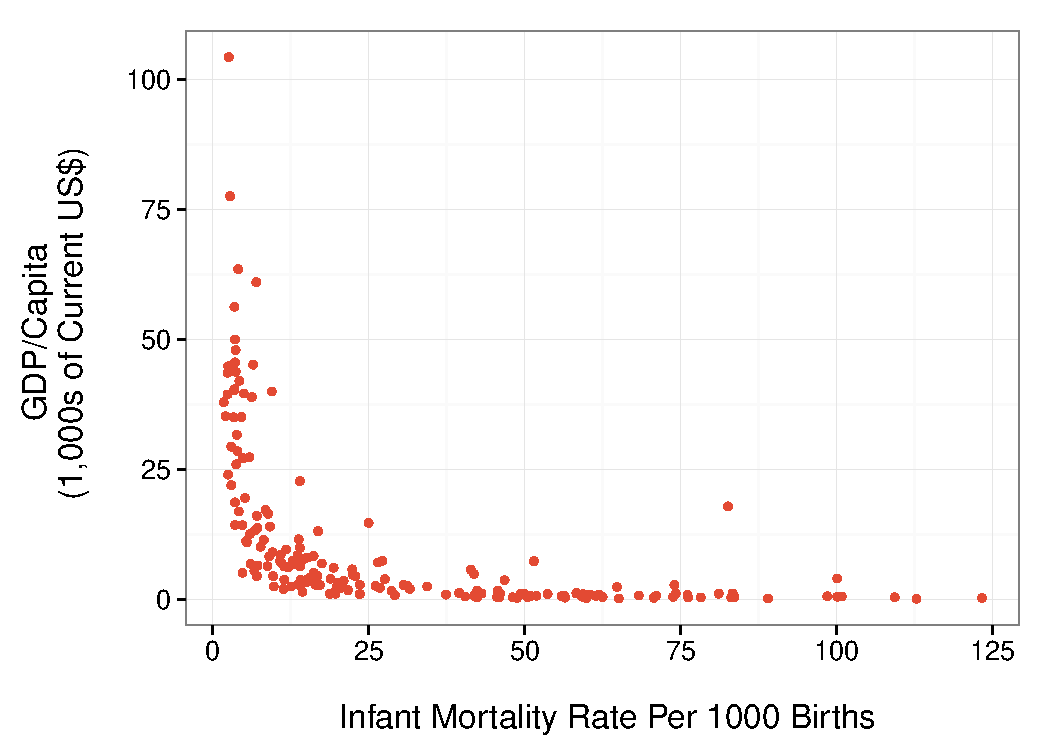
\includegraphics[width=\maxwidth]{figure/SimpleScatter} 

}


\end{knitrout}

\end{frame}

\frame{
  \frametitle{Tufte's Principles}
  {\LARGE{Goal of Statistical Graphics:}} \\[0.5cm]
  \begin{center}
    {\Large{The efficient communication of complex quantitative ideas.}}
  \end{center}
}

\frame{
  \frametitle{Tufte's Principles}
  {\LARGE{Tufte's Principles for Excellent Statistical Graphics (2001, 13) (a selection):}} \\[0.25cm]
  \begin{itemize}
    \item show the data
    \item encourage the eye to compare differences in the data
    \item serve a clear purpose
    \item avoid distorting the data
    \item be closely integrated with the text
  \end{itemize}
}

\frame{
  \frametitle{}
  \begin{center}
  {\LARGE{Show the Data \\[1cm]
  Encourage the eye to compare differences. \\[1cm]
  Serve a purpose.}}
  \end{center}
}

\frame{
  \frametitle{Show the data}
  {\Large{Show the data, not other things like silly graphics, or unnecessary words.}} \\[0.5cm]
  Have high {\bf{data ink}} ratio.
  \begin{equation}
    \mathrm{Data\:Ink\:Ratio = \frac{data-ink}{total\:ink}}
  \end{equation}
}

\frame{
  \frametitle{}
  \begin{center}
  {\LARGE{Example}}
  \end{center}
}

\frame{
  \frametitle{Encourge the Eye to Compare Differences}
  {\Large{How did the budgets change?}} \\
  \begin{center}
    (Orange is 2013, Blue is 2012) \\
    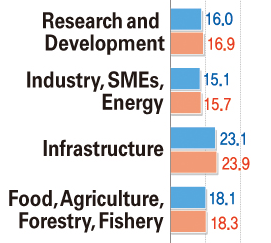
\includegraphics[scale=0.6]{figure/SpendingChange.png}
  \end{center}
}

\begin{frame}[fragile]
  \frametitle{A Little Better}



\begin{knitrout}
\definecolor{shadecolor}{rgb}{0.969, 0.969, 0.969}\color{fgcolor}

{\centering 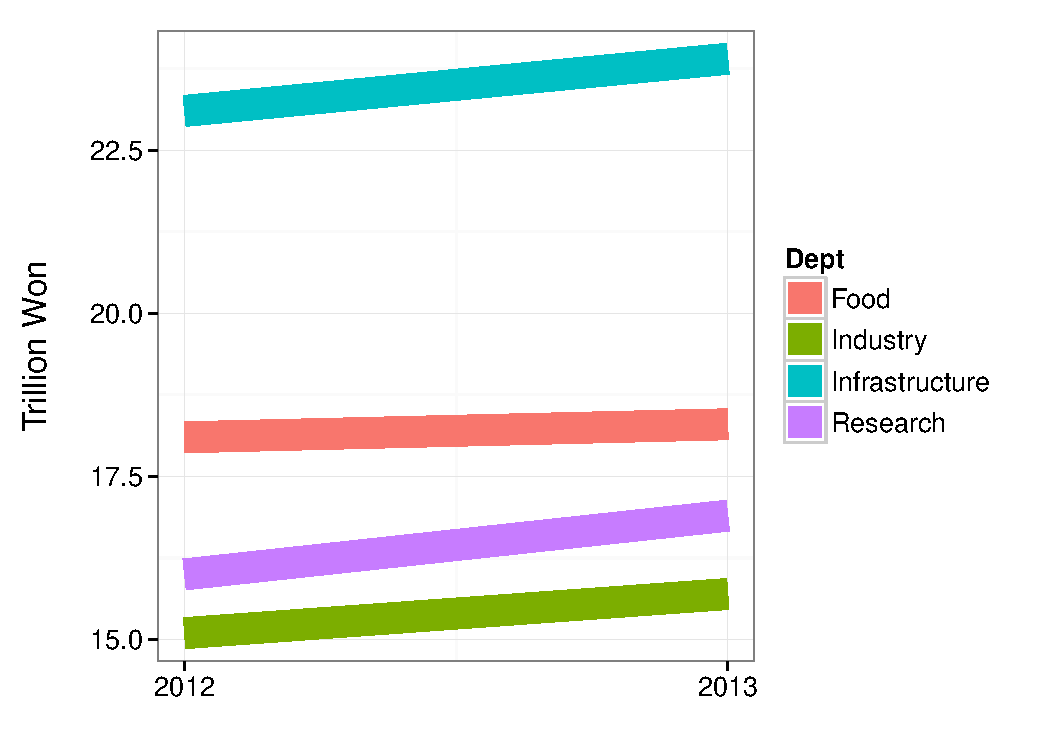
\includegraphics[width=\maxwidth]{figure/SpendingGraph} 

}


\end{knitrout}

\end{frame}

\begin{frame}[fragile]
  \frametitle{Even Better}



\begin{knitrout}
\definecolor{shadecolor}{rgb}{0.969, 0.969, 0.969}\color{fgcolor}

{\centering 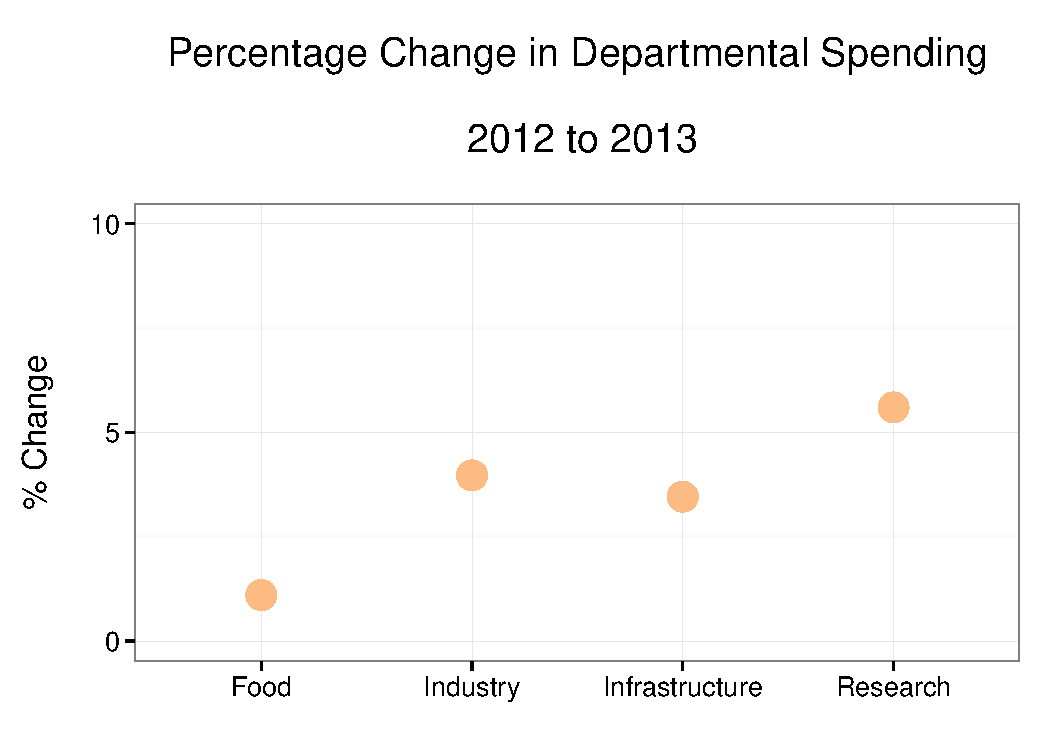
\includegraphics[width=\maxwidth]{figure/SpendPerChange} 

}


\end{knitrout}

\end{frame}


\frame{
  \frametitle{}
  \begin{center}
  {\LARGE{Avoid distorting the data.}} \\[1cm]
  Special case: Circles.
  \end{center}
}

\frame{
  \frametitle{Avoid Circles! (1)}
  \begin{center}
  {\Large{In general: Avoid using the {\emph{size}} of a circle to mean something!}}
  \end{center} \\[0.5cm]
  This includes avoiding:
  \begin{itemize}
    \item Bubble charts
    \item Pie charts
  \end{itemize}
}

\frame{
    \frametitle{Avoid Circles! (2)}
    {\Large{Why?}} \\[0.5cm]
    Circles can distort data.
    \begin{itemize}
      \item It is very difficult to compare their size
      \item The Ebbinghause Illusion!
    \end{itemize}
}

\frame{
  \frametitle{}
  Order the 4 circles from largest to smallest. \\[0.25cm]
  The circles are on a scale of 0-100, so how much bigger are each of the circles relative to each other? \\[0.25cm]
  \begin{center}
    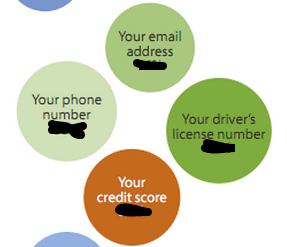
\includegraphics[scale=0.6]{figure/CirclesCompare.png}
  \end{center}
}

\begin{frame}[fragile]
  Order the 4 bars from largest to smallest. \\[0.25cm]
  How much bigger are each of the circles relative to each other? \\[0.25cm]




\begin{knitrout}
\definecolor{shadecolor}{rgb}{0.969, 0.969, 0.969}\color{fgcolor}

{\centering 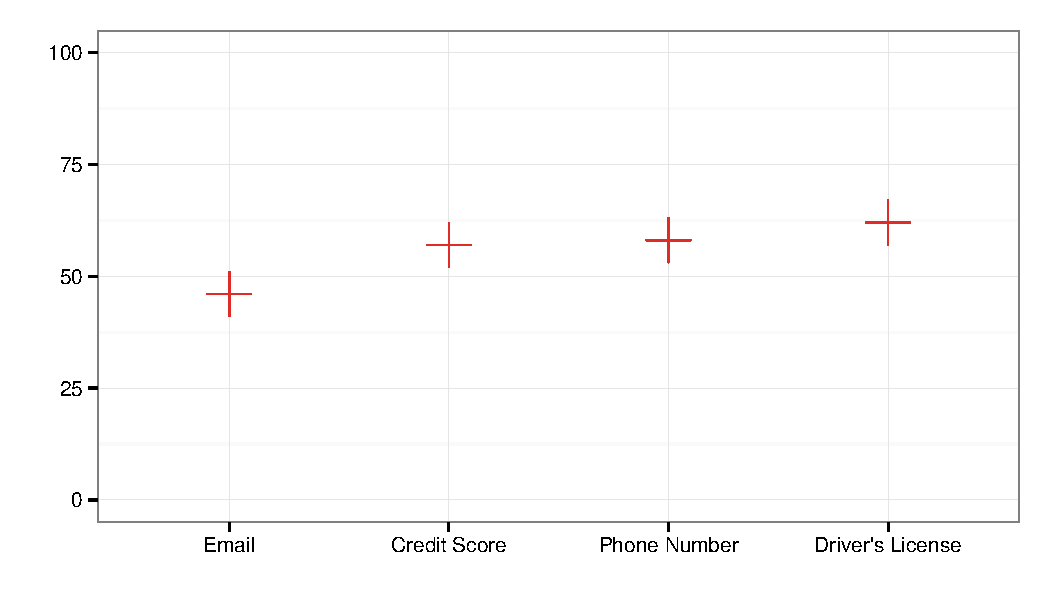
\includegraphics[width=\maxwidth]{figure/GraphCirclesComp} 

}


\end{knitrout}

\end{frame}

\frame{
  \frametitle{}
  {\Large{The circles basically tell you nothing that a simple table could do better.}}
  \begin{center}
    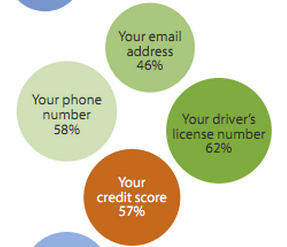
\includegraphics[scale=0.6]{figure/CirclesCompareNumbers.png}
  \end{center}
}

\frame{
  \frametitle{Ebbinghause Illusion}
  {\Large{Which circle is bigger?}}
  
\includegraphics[scale=0.6]{figure/Ebbinghause.png}
}

\frame{
  \frametitle{Another Issue}
  {\LARGE{Colour blindness.}}
}

\frame{
  \frametitle{Be colour blind friendly.}
  {\LARGE{ Colour blindness:}} \\[0.5cm]
  People who are colour blind can have difficulty distinquishing between red-green and blue-yellow. \\[0.25cm]
  About 5-8\% of men are colour blind. \\[0.25cm]
  We need to choose colour schemes for our graphics that are {\bf{colour blind friendly}}.\\[0.25cm]
  For more information see \url{http://www.usability.gov/articles/newsletter/pubs/022010new.html}.
}

\frame{
  \frametitle{Warning}
  {\LARGE{Remember:}} \\[0.5cm]
  {\Large{Graphics are only as good as what you put in them. \\[0.5cm]
  Silly data and statistics will always create silly graphs.}}
}

%%%%%%%%%%%%%%%%% Base R Graphics %%%%%%%%%%%%%
\frame{
  \frametitle{Base R Graphics}
  \begin{center}
    {\LARGE{Base R Graphics}}
  \end{center}
}

\frame{
  \frametitle{Base R Graphics}
  {\Large{Last week we saw that R has some basic graphics functions like:
  \begin{itemize}
    \item \texttt{plot}
    \item \texttt{histogram}
  \end{itemize}  
  }}
}
  

%%%%%%%%%%%%%%%%% Graphics with ggplot2 %%%%%%%%%%%%%
\frame{
  \frametitle{Graphics with gglot2}
  \begin{center}
    {\LARGE{Graphics with ggplot2}}
  \end{center}
}

\frame{
  \frametitle{Colours! (1)}
  {\LARGE{Colours}} \\[0.5cm]
  There are a number of ways to specify colours in ggplot2. \\[0.25cm]
  The simplest way is to let ggplot choose the colours for you.
}

\begin{frame}[fragile,plain]
\begin{knitrout}
\definecolor{shadecolor}{rgb}{0.969, 0.969, 0.969}\color{fgcolor}\begin{kframe}
\begin{alltt}
\hlcomment{# Create scatter plot divided by region}
\hlfunctioncall{ggplot}(data = InfantNoMiss, \hlfunctioncall{aes}(\hlfunctioncall{log}(InfantMortality),
                                \hlfunctioncall{log}(GDPperCapita))) +
      \hlfunctioncall{geom_point}(\hlfunctioncall{aes}(colour = income)) + 
      \hlfunctioncall{theme_bw}()
\end{alltt}
\end{kframe}

{\centering 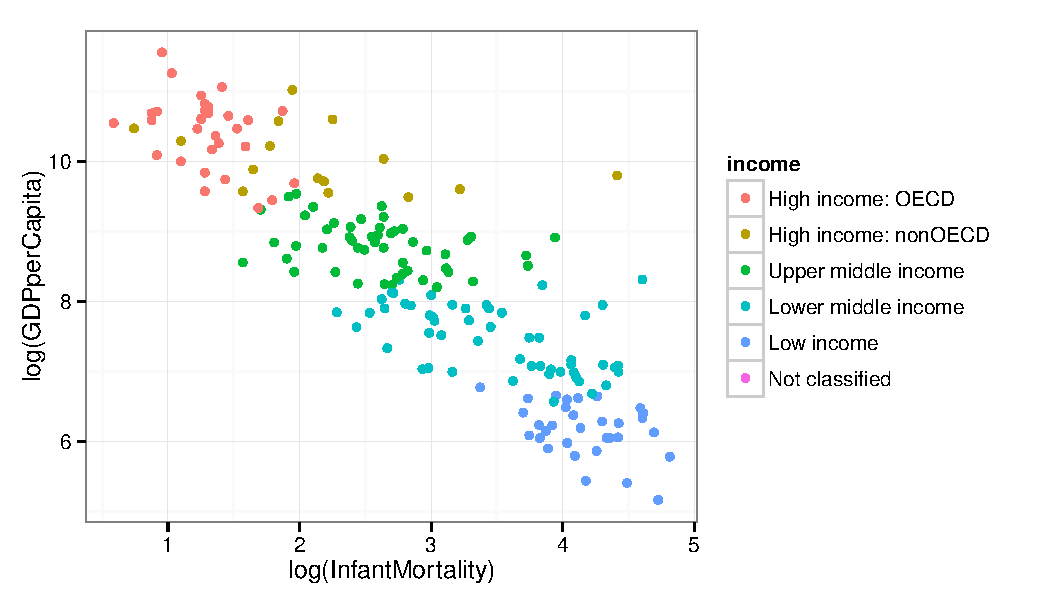
\includegraphics[width=\maxwidth]{figure/ScatterColour1} 

}


\end{knitrout}

\end{frame}

\begin{frame}[fragile]
  \frametitle{Colors! (2)}
  There are many ways to pick specific colors. \\[0.5cm]
  In this class we will mainly use {\bf{hexadecimal}} colours. \\[0,25cm]
  This is probably the most comonly used system for choosing colours on the web.\\[0.5cm]
  {\bf{Every}} colour is given six digits. \\[0.25cm]
  A good website for getting hexadecimal colour schemes is: \url{http://colorbrewer2.org/}.
\end{frame}

\begin{frame}[fragile,plain]
\begin{knitrout}
\definecolor{shadecolor}{rgb}{0.969, 0.969, 0.969}\color{fgcolor}\begin{kframe}
\begin{alltt}
\hlcomment{# Create colour vector}
Colours <- \hlfunctioncall{c}(\hlstring{"#1B9E77"}, \hlstring{"#D95F02"}, \hlstring{"#7570B3"}, 
             \hlstring{"#E7298A"}, \hlstring{"#66A61E"}, \hlstring{"#E6AB02"})

\hlcomment{# Create graph}
ColourScatter <- \hlfunctioncall{ggplot}(data = InfantNoMiss, 
                        \hlfunctioncall{aes}(\hlfunctioncall{log}(InfantMortality),
                            \hlfunctioncall{log}(GDPperCapita))) +
                  \hlfunctioncall{geom_point}(\hlfunctioncall{aes}(colour = income)) + 
                  \hlfunctioncall{scale_color_manual}(values = Colours) +
                  \hlfunctioncall{theme_bw}()
\end{alltt}
\end{kframe}
\end{knitrout}

\end{frame}

\begin{frame}[fragile,plain]
\begin{knitrout}
\definecolor{shadecolor}{rgb}{0.969, 0.969, 0.969}\color{fgcolor}\begin{kframe}
\begin{alltt}
\hlcomment{# Show scatter plot}
ColourScatter
\end{alltt}
\end{kframe}

{\centering 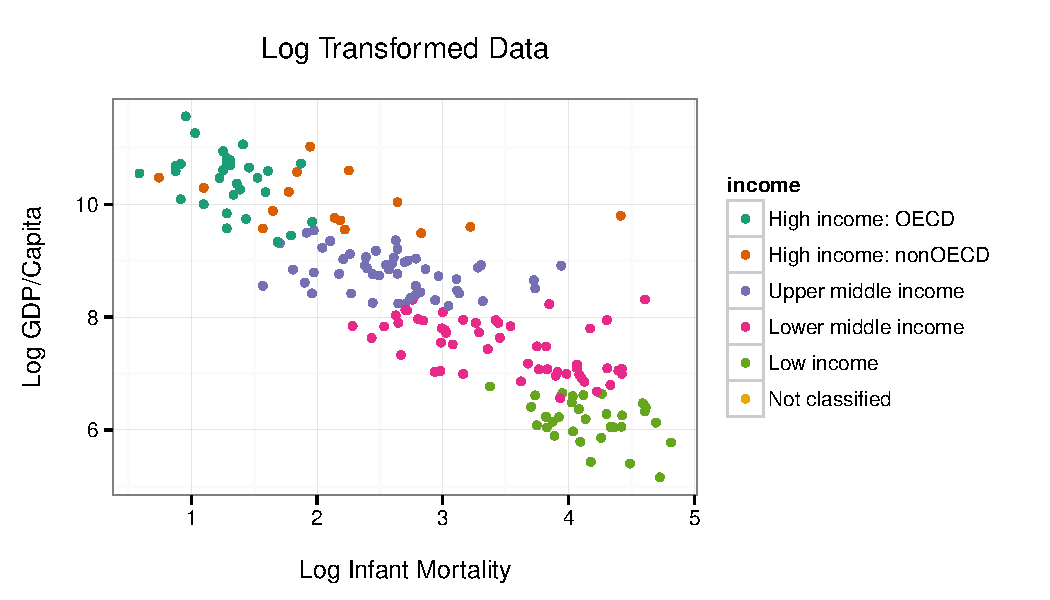
\includegraphics[width=\maxwidth]{figure/HexColoursScatter} 

}


\end{knitrout}


\end{frame}

%%%%%%%%%%%%%%%%% Graphics with GoogleVis %%%%%%%%%%%%%
\frame{
  \frametitle{Maps with gglot2}
  \begin{center}
    {\LARGE{Maps with ggplot2}}
  \end{center}
}


\frame{
  \frametitle{Professional Graphics With R}
  {\Large{Many people use R to create professional graphics. \\[0.5cm]
  For example: see the New York Times' graphics blog: \url{http://chartsnthings.tumblr.com/} \\[0.5cm]
  They often use R in combination with Adobe Illustrator. \\[0.5cm]
  See Nathan Yau's Book {\emph{Visualize This: The Flowing Data Guide to Design, Visualization, and Statistics}} (\url{http://book.flowingdata.com/}).
  }}
}

%%%%%%%% References
\begin{frame}[allowframebreaks]
  \frametitle{References}
  Tufte, Edward R. 2001. The Visual Display of Quantitative Information. Cheshire, Connecticut: Graphics Press.
 \\[0.25cm]
 
\end{frame}


\end{document}
